
%% bare_conf.tex
%% V1.4b
%% 2015/08/26
%% by Michael Shell
%% See:
%% http://www.michaelshell.org/
%% for current contact information.
%%
%% This is a skeleton file demonstrating the use of IEEEtran.cls
%% (requires IEEEtran.cls version 1.8b or later) with an IEEE
%% conference paper.
%%
%% Support sites:
%% http://www.michaelshell.org/tex/ieeetran/
%% http://www.ctan.org/pkg/ieeetran
%% and
%% http://www.ieee.org/

%%*************************************************************************
%% Legal Notice:
%% This code is offered as-is without any warranty either expressed or
%% implied; without even the implied warranty of MERCHANTABILITY or
%% FITNESS FOR A PARTICULAR PURPOSE! 
%% User assumes all risk.
%% In no event shall the IEEE or any contributor to this code be liable for
%% any damages or losses, including, but not limited to, incidental,
%% consequential, or any other damages, resulting from the use or misuse
%% of any information contained here.
%%
%% All comments are the opinions of their respective authors and are not
%% necessarily endorsed by the IEEE.
%%
%% This work is distributed under the LaTeX Project Public License (LPPL)
%% ( http://www.latex-project.org/ ) version 1.3, and may be freely used,
%% distributed and modified. A copy of the LPPL, version 1.3, is included
%% in the base LaTeX documentation of all distributions of LaTeX released
%% 2003/12/01 or later.
%% Retain all contribution notices and credits.
%% ** Modified files should be clearly indicated as such, including  **
%% ** renaming them and changing author support contact information. **
%%*************************************************************************


% *** Authors should verify (and, if needed, correct) their LaTeX system  ***
% *** with the testflow diagnostic prior to trusting their LaTeX platform ***
% *** with production work. The IEEE's font choices and paper sizes can   ***
% *** trigger bugs that do not appear when using other class files.       ***                          ***
% The testflow support page is at:
% http://www.michaelshell.org/tex/testflow/



\documentclass[conference]{IEEEtran}
% Some Computer Society conferences also require the compsoc mode option,
% but others use the standard conference format.
%
% If IEEEtran.cls has not been installed into the LaTeX system files,
% manually specify the path to it like:
% \documentclass[conference]{../sty/IEEEtran}





% Some very useful LaTeX packages include:
% (uncomment the ones you want to load)

% *** MISC UTILITY PACKAGES ***
%
%\usepackage{ifpdf}
% Heiko Oberdiek's ifpdf.sty is very useful if you need conditional
% compilation based on whether the output is pdf or dvi.
% usage:
% \ifpdf
%   % pdf code
% \else
%   % dvi code
% \fi
% The latest version of ifpdf.sty can be obtained from:
% http://www.ctan.org/pkg/ifpdf
% Also, note that IEEEtran.cls V1.7 and later provides a builtin
% \ifCLASSINFOpdf conditional that works the same way.
% When switching from latex to pdflatex and vice-versa, the compiler may
% have to be run twice to clear warning/error messages.






% *** CITATION PACKAGES ***
%
%\usepackage{cite}
% cite.sty was written by Donald Arseneau
% V1.6 and later of IEEEtran pre-defines the format of the cite.sty package
% \cite{} output to follow that of the IEEE. Loading the cite package will
% result in citation numbers being automatically sorted and properly
% "compressed/ranged". e.g., [1], [9], [2], [7], [5], [6] without using
% cite.sty will become [1], [2], [5]--[7], [9] using cite.sty. cite.sty's
% \cite will automatically add leading space, if needed. Use cite.sty's
% noadjust option (cite.sty V3.8 and later) if you want to turn this off
% such as if a citation ever needs to be enclosed in parenthesis.
% cite.sty is already installed on most LaTeX systems. Be sure and use
% version 5.0 (2009-03-20) and later if using hyperref.sty.
% The latest version can be obtained at:
% http://www.ctan.org/pkg/cite
% The documentation is contained in the cite.sty file itself.






% *** GRAPHICS RELATED PACKAGES ***
%
\ifCLASSINFOpdf
  % \usepackage[pdftex]{graphicx}
  % declare the path(s) where your graphic files are
  % \graphicspath{{../pdf/}{../jpeg/}}
  % and their extensions so you won't have to specify these with
  % every instance of \includegraphics
  % \DeclareGraphicsExtensions{.pdf,.jpeg,.png}
\else
  % or other class option (dvipsone, dvipdf, if not using dvips). graphicx
  % will default to the driver specified in the system graphics.cfg if no
  % driver is specified.
  % \usepackage[dvips]{graphicx}
  % declare the path(s) where your graphic files are
  % \graphicspath{{../eps/}}
  % and their extensions so you won't have to specify these with
  % every instance of \includegraphics
  % \DeclareGraphicsExtensions{.eps}
\fi
% graphicx was written by David Carlisle and Sebastian Rahtz. It is
% required if you want graphics, photos, etc. graphicx.sty is already
% installed on most LaTeX systems. The latest version and documentation
% can be obtained at: 
% http://www.ctan.org/pkg/graphicx
% Another good source of documentation is "Using Imported Graphics in
% LaTeX2e" by Keith Reckdahl which can be found at:
% http://www.ctan.org/pkg/epslatex
%
% latex, and pdflatex in dvi mode, support graphics in encapsulated
% postscript (.eps) format. pdflatex in pdf mode supports graphics
% in .pdf, .jpeg, .png and .mps (metapost) formats. Users should ensure
% that all non-photo figures use a vector format (.eps, .pdf, .mps) and
% not a bitmapped formats (.jpeg, .png). The IEEE frowns on bitmapped formats
% which can result in "jaggedy"/blurry rendering of lines and letters as
% well as large increases in file sizes.
%
% You can find documentation about the pdfTeX application at:
% http://www.tug.org/applications/pdftex





% *** MATH PACKAGES ***
%
%\usepackage{amsmath}
% A popular package from the American Mathematical Society that provides
% many useful and powerful commands for dealing with mathematics.
%
% Note that the amsmath package sets \interdisplaylinepenalty to 10000
% thus preventing page breaks from occurring within multiline equations. Use:
%\interdisplaylinepenalty=2500
% after loading amsmath to restore such page breaks as IEEEtran.cls normally
% does. amsmath.sty is already installed on most LaTeX systems. The latest
% version and documentation can be obtained at:
% http://www.ctan.org/pkg/amsmath





% *** SPECIALIZED LIST PACKAGES ***
%
%\usepackage{algorithmic}
% algorithmic.sty was written by Peter Williams and Rogerio Brito.
% This package provides an algorithmic environment fo describing algorithms.
% You can use the algorithmic environment in-text or within a figure
% environment to provide for a floating algorithm. Do NOT use the algorithm
% floating environment provided by algorithm.sty (by the same authors) or
% algorithm2e.sty (by Christophe Fiorio) as the IEEE does not use dedicated
% algorithm float types and packages that provide these will not provide
% correct IEEE style captions. The latest version and documentation of
% algorithmic.sty can be obtained at:
% http://www.ctan.org/pkg/algorithms
% Also of interest may be the (relatively newer and more customizable)
% algorithmicx.sty package by Szasz Janos:
% http://www.ctan.org/pkg/algorithmicx




% *** ALIGNMENT PACKAGES ***
%
%\usepackage{array}
% Frank Mittelbach's and David Carlisle's array.sty patches and improves
% the standard LaTeX2e array and tabular environments to provide better
% appearance and additional user controls. As the default LaTeX2e table
% generation code is lacking to the point of almost being broken with
% respect to the quality of the end results, all users are strongly
% advised to use an enhanced (at the very least that provided by array.sty)
% set of table tools. array.sty is already installed on most systems. The
% latest version and documentation can be obtained at:
% http://www.ctan.org/pkg/array


% IEEEtran contains the IEEEeqnarray family of commands that can be used to
% generate multiline equations as well as matrices, tables, etc., of high
% quality.




% *** SUBFIGURE PACKAGES ***
%\ifCLASSOPTIONcompsoc
%  \usepackage[caption=false,font=normalsize,labelfont=sf,textfont=sf]{subfig}
%\else
%  \usepackage[caption=false,font=footnotesize]{subfig}
%\fi
% subfig.sty, written by Steven Douglas Cochran, is the modern replacement
% for subfigure.sty, the latter of which is no longer maintained and is
% incompatible with some LaTeX packages including fixltx2e. However,
% subfig.sty requires and automatically loads Axel Sommerfeldt's caption.sty
% which will override IEEEtran.cls' handling of captions and this will result
% in non-IEEE style figure/table captions. To prevent this problem, be sure
% and invoke subfig.sty's "caption=false" package option (available since
% subfig.sty version 1.3, 2005/06/28) as this is will preserve IEEEtran.cls
% handling of captions.
% Note that the Computer Society format requires a larger sans serif font
% than the serif footnote size font used in traditional IEEE formatting
% and thus the need to invoke different subfig.sty package options depending
% on whether compsoc mode has been enabled.
%
% The latest version and documentation of subfig.sty can be obtained at:
% http://www.ctan.org/pkg/subfig




% *** FLOAT PACKAGES ***
%
%\usepackage{fixltx2e}
% fixltx2e, the successor to the earlier fix2col.sty, was written by
% Frank Mittelbach and David Carlisle. This package corrects a few problems
% in the LaTeX2e kernel, the most notable of which is that in current
% LaTeX2e releases, the ordering of single and double column floats is not
% guaranteed to be preserved. Thus, an unpatched LaTeX2e can allow a
% single column figure to be placed prior to an earlier double column
% figure.
% Be aware that LaTeX2e kernels dated 2015 and later have fixltx2e.sty's
% corrections already built into the system in which case a warning will
% be issued if an attempt is made to load fixltx2e.sty as it is no longer
% needed.
% The latest version and documentation can be found at:
% http://www.ctan.org/pkg/fixltx2e


%\usepackage{stfloats}
% stfloats.sty was written by Sigitas Tolusis. This package gives LaTeX2e
% the ability to do double column floats at the bottom of the page as well
% as the top. (e.g., "\begin{figure*}[!b]" is not normally possible in
% LaTeX2e). It also provides a command:
%\fnbelowfloat
% to enable the placement of footnotes below bottom floats (the standard
% LaTeX2e kernel puts them above bottom floats). This is an invasive package
% which rewrites many portions of the LaTeX2e float routines. It may not work
% with other packages that modify the LaTeX2e float routines. The latest
% version and documentation can be obtained at:
% http://www.ctan.org/pkg/stfloats
% Do not use the stfloats baselinefloat ability as the IEEE does not allow
% \baselineskip to stretch. Authors submitting work to the IEEE should note
% that the IEEE rarely uses double column equations and that authors should try
% to avoid such use. Do not be tempted to use the cuted.sty or midfloat.sty
% packages (also by Sigitas Tolusis) as the IEEE does not format its papers in
% such ways.
% Do not attempt to use stfloats with fixltx2e as they are incompatible.
% Instead, use Morten Hogholm'a dblfloatfix which combines the features
% of both fixltx2e and stfloats:
%
% \usepackage{dblfloatfix}
% The latest version can be found at:
% http://www.ctan.org/pkg/dblfloatfix




% *** PDF, URL AND HYPERLINK PACKAGES ***
%
%\usepackage{url}
% url.sty was written by Donald Arseneau. It provides better support for
% handling and breaking URLs. url.sty is already installed on most LaTeX
% systems. The latest version and documentation can be obtained at:
% http://www.ctan.org/pkg/url
% Basically, \url{my_url_here}.




% *** Do not adjust lengths that control margins, column widths, etc. ***
% *** Do not use packages that alter fonts (such as pslatex).         ***
% There should be no need to do such things with IEEEtran.cls V1.6 and later.
% (Unless specifically asked to do so by the journal or conference you plan
% to submit to, of course. )


% correct bad hyphenation here
\hyphenation{op-tical net-works semi-conduc-tor}


% Inserted by Eduardo
\usepackage{color}
\usepackage[]{algorithm}

% Inserted by Bernardo
\usepackage[noend]{algpseudocode}
\usepackage{listings}
\usepackage{subcaption}
\usepackage{graphicx}
\usepackage{amsmath}
\usepackage[utf8]{inputenc}
\usepackage{tikz}
\usetikzlibrary{positioning}
\usepackage{pgfplots}

\lstdefinestyle{mystyle}{
  basicstyle=\ttfamily\tiny,
  breaklines=true,
  keepspaces=true,
  keywords={Input,Output,for,if,while,do,end,in,def,and,or,return},
  tabsize=2
}
\lstset{style=mystyle}

\algnewcommand\algorithmicforeach{\textbf{for each}}
\algdef{S}[FOR]{ForEach}[1]{\algorithmicforeach\ #1\ \algorithmicdo}

\begin{document}
%
% paper title
% Titles are generally capitalized except for words such as a, an, and, as,
% at, but, by, for, in, nor, of, on, or, the, to and up, which are usually
% not capitalized unless they are the first or last word of the title.
% Linebreaks \\ can be used within to get better formatting as desired.
% Do not put math or special symbols in the title.
\title{Maximizing the GPU Resource Usage by Reordering Concurrent Kernels Submission}



% conference papers do not typically use \thanks and this command
% is locked out in conference mode. If really needed, such as for
% the acknowledgment of grants, issue a \IEEEoverridecommandlockouts
% after \documentclass

% for over  affiliations, or if they all won't fit within the width
% of the page, use this alternative format:
% 
\author{\IEEEauthorblockN{
Bernardo Breder\IEEEauthorrefmark{1},
Eduardo Charles\IEEEauthorrefmark{1},
Rommel Cruz\IEEEauthorrefmark{1}, 
Esteban Clua\IEEEauthorrefmark{1} and
Cristiana Bentes\IEEEauthorrefmark{2}
Lucia Drummond\IEEEauthorrefmark{1}}
\IEEEauthorblockA{\IEEEauthorrefmark{1}Institute of Computing\\
Federal Fluminense University,
RJ - Brazil, 24210-240 \\ 
Email: {bernardo,eduardo,rommel,esteban,lucia}@ic.uff.br}
\IEEEauthorblockA{\IEEEauthorrefmark{2}Department of System Engineering \\
State University of Rio de Janeiro,
RJ - Brazil, 20550-900\\
Email: cris@eng.uerj.br}
}




% use for special paper notices
%\IEEEspecialpapernotice{(Invited Paper)}




% make the title area
\maketitle

% As a general rule, do not put math, special symbols or citations
% in the abstract
\begin{abstract}
The increasing amount of resources available on current GPUs sparked new interest in the problem of sharing its resources by different kernels. While new generation of GPUs support concurrent kernel execution, their scheduling decisions are taken by the hardware at runtime. The hardware decisions, however, heavily depends on the order
at which the kernels are submitted to execution. In this work, we propose a novel optimization approach to reorder the kernels invocation focusing on maximizing the resources utilization, improving the average execution time. We model the kernels assignments to the hardware resources as a series of knapsack problems and use dynamic programming approach to solve them. We evaluate our method using kernels with different sizes and resource requirements. Our results show significant gains in the resource usage and in the average execution time compared to the naive kernels submission implemented in modern GPUs.
\end{abstract}

% no keywords




% For peer review papers, you can put extra information on the cover
% page as needed:
% \ifCLASSOPTIONpeerreview
% \begin{center} \bfseries EDICS Category: 3-BBND \end{center}
% \fi
%
% For peerreview papers, this IEEEtran command inserts a page break and
% creates the second title. It will be ignored for other modes.
\IEEEpeerreviewmaketitle

\section{Introduction}
\label{sec:Introduction}

Graphics Processing Units (GPUs) are increasingly popular these days due to their higher performance and lower energy consumption compared to traditional multicore CPUs. GPUs support a massive amount of parallelism at relatively low cost. The practice of offloading computation to run on GPUs provides significant acceleration for a wide range of arithmetic-intensive data-parallel applications. 

In the case of NVIDIA GPUs and the CUDA programming model, \textit{kernels} are offloaded to the GPU. The kernel code is executed by multiple parallel threads running on different GPU cores. The programmer organizes the threads into thread {\it blocks}, and the GPU architecture divides the cores into sets of Streaming Multiprocessors (SMs). Thread blocks are created at runtime, and the GPU scheduler assigns each block to a specific SM for execution. A thread block cannot migrate between SMs after it is scheduled. 

In face of the increasing amount of resources available on current GPUs and the advances in their microarchitecture, an emerging challenge is how to share effectively the GPU resources by different kernels. There were expressive growth in core count, shared memory, registers and hardware threads, but many applications are not ready to take advantage of all these resources.  According to Pai \textit{et al.} \cite{pai2013improving}, the Parboil2 benchmark suite uses only from 20\% to 70\% of the Fermi GPU resources. Adriens \textit{et al.} \cite{adriaens2012case} performs similar studies for 12 real-world applications, and show that most of them exhibit unbalanced GPU resource utilization.

In order to better utilize the GPU hardware resources, new generation NVIDIA GPUs support concurrent kernel execution.  Initially introduced in the Fermi architecture, concurrent kernel execution was somewhat restrictive. Programmers specify kernels independence -- by placing them on different CUDA streams -- and the hardware multiplexes the kernels into a work queue. Up to 16 kernels from different streams can execute simultaneously~\cite{FermiArch:2010}. While this feature was beneficial for increasing the GPU utilization, there were limitations: (i) only  kernels of the same application can execute concurrently, and (ii) the issue order to the work queue matters for concurrency, it can cause \textit{false-serialization} (if the kernel $k_j$ that follows kernel $k_i$ on the queue are on the same stream, they will be serialized in the execution). Later, the Kepler architecture tackled these limitations by providing the Hyper-Q technology, where up to 32 hardware queues enable multiple applications running on different CPU cores to simultaneously utilize the GPU resources.

The Hyper-Q technology allows threads blocks from different streams to share the same resources in the GPU. For example, consider a recent GPU architecture with XX registers, XX of shared memory, and a maximum of 2048 threads per SM. Also consider a kernel $k_i$ with 2 thread blocks, each block containing 512 threads and using $1/4$ of the shared memory, and each thread using XX registers. In this scenario, the SM will have unused resources: half of the maximum threads, half of the shared memory and half of the registers. These unused resources can be allocated to other thread blocks from different kernels (placed on different streams).

The NVIDIA scheduling policy is proprietary, and no information has been made available by them about. There is, however, some speculation that the scheduling policy follows a \textit{left-over} strategy \cite{pai2013improving}. The scheduler dispatches the blocks from the first kernel in the first queue, if there are still available resources, blocks from the kernels of the next queues are also dispatched in a round-robin fashion. Two kernels from the same queue, however, are dispatched in sequential order. The problem with this scheduling policy is that the order at which the kernels were inserted on the queues has significant impact on the GPU occupancy. Suppose the example of Figure \ref{fig:occupancy}, where four kernels on different streams were submitted to run. Each kernel requests a different amount of resources and has different execution times. In Figure~\ref{fig:occupancy} (a) we show their execution considering the submission order $\{k_1, k_2, k_3, k_4\}$. According to the NVIDIA scheduler kernel $k_1$ is submitted first, and kernel $k_2$ is also submitted due to the left-over policy. When $k_2$ finishes, $k_3$ is submitted, but $k_4$ has to wait because its resource request is not available. We can observe that from $t_0$ to $t_1$ there are 40\% of the resources still available, and from $t_2$ to $t_3$ there are 50\% available. If we consider a different order to submit the kernels, and submit in the following order $\{k_4, k_1, k_3, k_2\}$, the NVIDIA scheduler will execute the kernels as shown in Figure~\ref{fig:occupancy} (b). We can observe that until $t_3$ there are at most 20\% of the resources available, which improves significantly the resource usage. 

\begin{figure}[htb]
\centering
\includegraphics[width=3.5in,height=1.9in]{scheduling2.eps}
\caption{A set of four kernels is submitted to the GPU in two orders. In (a) the submission order is $\{k_1, k_2, k_3, k_4\}$. In (b) the submission order is $\{k_4, k_1, k_3, k_2\}$}
\label{fig:occupancy}
\end{figure}

In this work, we propose an optimization strategy that determines the order to submit the kernels for the GPU queues. The idea is to simulate the assignment of kernels to the hardware queues in order to maximize the resources utilization, improving the overall throughput. Our approach models the problem of selecting which kernels are better to submit to take the most advantage of the available resources as a series of knapsack problems. We model the set of the available resources as the knapsack capacity and the set of kernels as the items to be put into the knapsack. The kernels have weights and values 
according to the amount of resource usage -- shared memory, number of register and number of threads -- and the estimated execution time. The solution to the knapsack problem establishes the subset of kernels whose total weight is smaller than the available resources and the total value is as large as possible. We use a dynamic programming algorithm to solve the knapsack problem and the algorithm outputs a reordering of the kernel submissions that maximizes the resource utilization. Our reordering algorithm targets applications composed on many “heavy” kernels (i.e. kernels with large computational time) that have different resources requirements. For this reason, the combinatorial optimization problem we are facing has a limited number of items and executes in negligible time.  We present results XXX.

The remainder of this paper is organized as follows.
Section~\ref{sec:Related} presents previous work on GPU concurrent kernel execution.
Section~\ref{sec:ProblemDefinition} gives a brief introduction to the problem we are facing and describes the proposed scheduling algorithm.
Section~\ref{sec:Results} presents the experimental results using synthetic and real-world problems. 
Finally, section~\ref{sec:Conclusions} draws some conclusions and presents future research directions.


\section{Related Work}
\label{sec:Related}

Before the GPU had the hardware support to execute different kernels concurrently, there were some efforts in overcoming this limitation in software by \textit{merging} the source of different kernels into one kernel to execute them concurrently.  The work of Guevara \textit{et al.} \cite{guevara2009enabling}  proposes a compile-time system that merges two kernels into a single kernel, what they call \textit{thread interleaving}. Peters \textit{et al.} \cite{peters2010efficiently} proposed a persistent kernel (with a fixed number of thread blocks) that can execute different functions written to the GPU memory concurrently. In this way, it is possible to handle requests from different applications. Recent GPU generations (eg, NVIDIA Fermi, Kepler and Maxwell) have already the ability to launch several kernels concurrently. The work of Wang \textit{et al.} \cite{wang2011exploiting}  addresses a limitation of the Fermi architecture in that all the concurrent kernels must come from the same application. Their approach, called \textit{context funneling}, is similar to kernel merging, but uses kernels from different contexts. However, kernels with different features, such as computational intensive or memory bound, are treated equally at scheduling. The work by Gregg \textit{et al.} \cite{gregg2012fine} proposes an OpenCL concurrent kernel scheduler that uses \textit{thread interleaving}. They combine two OpenCL dispatch operations into a single dispatch that launches the scheduler. The scheduler implements a queue and the thread blocks from the two kernels are put on the queue according to the scheduling algorithms: (i) round-robin with work-stealing and (ii) partitioning by kernel (ensures that the percentage of the resources assigned to each kernel remains fixed). Wang \textit{et al.} \cite{wang2010kernel} proposed \textit{kernel fusion}. Their focus, however, was on reducing energy consumption and improving power efficiency. Merging kernels at the source code or at the runtime circumvents by software some hardware limitations in launching concurrent kernels, but they do not consider the different resource requirements by the kernels.

On a different direction, some authors propose mechanisms to modify the granularity of the kernels, {\it slicing} them, in order to improve the GPU utilization. Zhong \textit{et al.} \cite{zhong2014kernelet} proposed to slice the kernel to create more opportunities for time sharing. They used a greedy algorithm to schedule the slices. Ravi \textit{et al.} \cite{ravi2011supporting} proposed the \textit{molding} technique that allows the changing of the dimensions of grid and thread blocks, but the kernel code has to accept this variation. Pai \textit{et al.} \cite{pai2013improving} improved this technique, proposing the \textit{elastic kernel}, that elasticizes any kind of kernel. They also proposed different elastic-kernel aware concurrency management policies. XXX (explicar das políticas aqui). For real-time applications, the works of Tanasic  \textit{et al.} \cite{tanasic2014enabling} and Park \textit{et al.} \cite{park2015chimera} proposed the implementation of preemption in the concurrent kernel execution.

There are also efforts in dividing the GPU resources among the concurrent kernels, called \textit{spatial multitasking}. These efforts, however, focus on proposing hardware enhancements to improve GPU utilization. The work by Liang \textit{et al.} \cite{liang2015efficient} uses the CUDA profiler to determine the amount of global memory requested for each kernel, and computes the kernel behavior in terms of latency and memory bandwidth by executing each kernel with a dummy counterpart. Their approach focus not only on partitioning the SMs among the kernels, but on deciding which kernels execute concurrently. They use a heuristic approach based on dynamic programming to divide the SMs and select the kernels for concurrent execution. Their spatial division, however, is not currently supported by the hardware. Their framework to emulate the GPU execution can modify the register usage, which can impact the results. Adriens \textit{et al.} \cite{adriaens2012case} show that GPU applications have unbalanced resource utilization and also show through simulation that statically partitioning the GPU resources among applications offers performance benefits. They propose four partition schemes to divide the GPU multiprocessors (SMs) among the applications: (i) Even: divides the SMs evenly; (ii) Smart Even: divides evenly, but without assigning more SMs than the application needs; (iii) Round:  defines a round as the execution of a group of thread blocks that starts and finishes at about the same time, and divides the SMs evenly guaranteeing that no application takes more rounds to execute than it would require; and (iv) Profile: profiles the application execution previously using different number of SMs, and divides the SMs according to the maximization of the application speedups. Their static division, however, does not take into account other resource usage rather than the SMs.

Closer to our work are the proposals that focus on achieving maximum utilization based the order in which GPU kernels are invoked on the host side, called \textit{kernel reordering}. Wende \textit{et al.} \cite{wende2012improving} propose kernel reordering for the Fermi hardware, where the concurrent kernel execution uses only one scheduling queue. They create a scheduler thread that arranges the scheduling queue in a round-robin fashion, without considering the threads resource utilization. They were successful in increasing the concurrency by interleaving different streams of execution in the same queue, but modern GPUs hardware have the Hyper-Q mechanism, that implements these queues in hardware. Our work is closest to the work of Li \textit{et al.} \cite{li2015power} that proposes a reordering scheme for further GPU architectures with Hyper-Q technology available. Their approach computes a \textit{symbiotic score}, that tries to co-execute kernels with complementary resource usage and predicted power consumption using the concept of \textit{execution rounds} -- round of simultaneous thread block execution on the SMs. They try to fulfill a round with symbiotic kernels using a greedy algorithm for the problem of multi-dimensional bin-packing. The use of rounds of execution simplify the scheduling decisions. In contrast, our reordering solution avoids the implicit synchronization of the round completion by solving a more complex problem each time there are available resources. 

 

% Cris: Rommel, esta tabela me parece desnecessária no paper. 
%Talvez na tese valha uma tabela parecida, mas que os aspectos levantados sejam diferenciados pelos trabalhos anteriores. Nas colunas que voce colocou todos os trabalhos possuem os aspectos levantados.
% Eu colocaria as seguintes colunas: (1) Work; (2) Strategy (diferenciar entre Kernel Merging, Kernel Slicing e Kernel Reordering; (3) Hardware (falar qual a geração da placa usada para experimentos/implementacao (Fermi, Kepler ou Maxwell) e colocar qual o suporte de hardware para escalonamento (No support, CKE, Hyper-Q); (4) Applications (qual benchmark suite foi usada nos testes).

%\begin{table*}[t]
%	\centering
%    \begin{minipage}{\textwidth}
%    \def\arraystretch{1.2}%
%	\begin{tabular}{lcccc}
%		\toprule
%		\multicolumn{1}{c}{Work} & Strategy & Target 	& Concurrent Kernel	& Test\\
%		                         & 			& hardware  & HW support 	& applications\\
%		\midrule
%		(Guevara et al., 2009) \cite{guevara2009enabling}         &	Merging & Tesla K20 (Kepler) Sim & Hyper-Q & 10 Parboil benchmark applications: LBM, Histo, TPACF, SPMV\\
%		& & & & MRI-Q, SAD, SGEMM, Stencil, CUTCP, MRI-gridding\\
%        (Wang et al., 2010) \cite{wang2010kernel}         &	Merging & Quadro FX 5800 (Tesla) & No support & Two CUDA applications: BlackScholes (CUDA SDK), \\
%        & & Simulated & & Swim (ported from SPEC2K CPU benchmark) \\
%        (Peters et al., 2010) \cite{peters2010efficiently}         &	Merging & GTX 260, 280 (Tesla) & No support & Two GPGPU applications: MatMul and Sorting\\
%		(Ravi et al., 2011) \cite{ravi2011supporting}             &	Merging & Tesla C2050 (Fermi) & Up to 16 & 8 GPGPU applications: Image Processing, \\
%        & & & & PDE Solver, BlackScholes, Binomial Options, K-Means, \\
%        & & & & K-Nearest Neighbours, Euler, Molecular Dynamics \\
%		(Wang et al., 2011) \cite{wang2011exploiting}             &	Merging & Tesla C2070 (Fermi) & Up to 16 & Microbenchmarsks and a GPGPU application:\\
%		& & & & Scalable Synthetic Compact Application \\
%        (Adriaens et al., 2012) \cite{adriaens2012case}           &	Reordering & Quadro FX 5800 (Tesla) & No support & 10 open source GPGPU applications: Ray Tracing \\
%        & & Simulated & & AES, RSA, SHA1, JPEG Encoding \& Decoding, Fractals\\
%        & & & & Image Denoising, Radix Sort, DVC, SAD (Parboil benchmark)\\
%		(Gregg et al., 2012) \cite{gregg2012fine}                 &	Merging & GTX 460 (Fermi) & Up to 16 & Bitonic Sort, Kmeans, Floyd Warshall \\
%		& & & & Nearest Neighbor, Simple Convolution, Fast Walsh Transform \\
%		(Wende et al., 2012) \cite{wende2012improving}            & Reordering	& Tesla M2090 (Fermi) & Up to 16 & Molecular dynamics simulation \\
        
		%(Awatramani et al., 2013) \cite{awatramani2013increasing} & HW novo & X & X & \\
%		(Pai et al., 2013) \cite{pai2013improving}                & Slicing & Tesla C2070 (Fermi) & Up to 16 & All Parboil2 benchmark kernels \\
%		(Zhong et al., 2014) \cite{zhong2014kernelet}             & Slicing	& Tesla C2050 (Fermi) & Up to 16 & 8 GPGPU applications from CUDA SDK, \\
%		& & GTX 680 (Kepler) & Hyper-Q & Parboil Benchmark and CUSP \\
		%(Tanasic et al., 2014) \cite{tanasic2014enabling}         & Preemptive	& X & X & \\
%		(Jiao et al., 2015) \cite{jiao2015improving}              &	Slicing & GTX 640 (Kepler) & Hyper-Q & 11 applications from the CUDA SDK\\
% 		& & & & and Rodinia Benchmark\\
		%(Park et al., 2015) \cite{park2015chimera}                & Preemptive	& X & X & \\
%		(Liang et al., 2015) \cite{liang2015efficient}			  &	Reordering & Tesla K20 (Kepler) & Hyper-Q & 9 CUDA SDK applications: VectorAdd, BinomialOptions \\
%		& & & & BlackScholes, Histogram256, MergeSort, Scan \\
%		& & & & Histogram64, Monte-CarloSim, FastWalshTransform \\
%		(Li et al., 2015) \cite{li2015power}                      & Reordering & Tesla K20 (Kepler) & Hyper-Q & 4 GPGPU applications: BlackScholes, SmithWaterman algorithm \\
%   		& & & & Electrostatics algorithm, Embarrassingly Parallel (NPB benchmark) \\
%	\bottomrule
%	\end{tabular}
%\end{minipage}%
%	\caption{GPU scheduling techniques}
%	\label{tab:tableRelatedWork}
%\end{table*}

\section{Problem Definition}
\label{sec:ProblemDefinition}

For a given GPU device, $D$, let $Ord=\{k_0, k_1, ..., k_{N-1}\}$ be the list of $N$ independent kernels in the order at which they are submitted for execution on $D$ ($k_i$ is submitted before $k_{i+1}$). Consider that $D$ has the resources $R_j \mid j \in \{0,1,2\}$, where: 

% XXXX - Precisamos definir a variável NSM que significa o número de stream multi-processor. Essa variável é utilizada no algoritmo.

\begin{itemize}
    \item $R_{0}$ is the shared memory size per SM;
    \item $R_{1}$ is the number of registers per SM;
    \item $R_{2}$ is the maximum supported number of threads per SM.
\end{itemize}


At a certain time during the execution, there are $m$ kernels executing concurrently on $D$, using a percentage of $R_j$. The available resources at this time are called $R_{j}^{av} \mid j \in \{0, 1, 2\}$. 

Every time $t_k^{free}$ a kernel finishes and releases resources, new kernels are selected for execution according to the amount of available resources.

In order to find a new submission order, $Ord^{new}$, so that the resource utilization is maximized, we model the problem of selecting a number of new kernels to submit and take advantage of the available resources as a multidimensional knapsack problem. In the model, at the beginning of the execution and at each $t_k^{free}$, $D$ represents the knapsack with the capacity equal to the available resources, and the non-submitted kernels represent the items to be packed into the knapsack. 

For each non-submitted kernel $k_i$, we collect the following information:
\begin{itemize}
    \item $t^{est}_{i}$: the estimated execution time;
    \item $sh_i$: the percentage of shared memory required per block;
    \item $nr_i$: the percentage of registers required per block; 
    \item $nt_i$: the percentage of the maximum number of threads launched per block. 
\end{itemize}

%\textcolor{red}{
%[Bernardo] - \'E poss\'ivel criar uma vari\'avel para quantidade de memoria compartilhada, registradores e n\'umero de threads ? Essas variaveis sao importante para o calculo do peso que não leva em consideracao a porcentagem e sim a quantidade. No algoritmo eu estou reconvertendo a porcentagem para o numero para que eu consiga o valor da quantidade. Como:
%\begin{itemize}
  %  \item $t^{est}_{i}$: the estimated execution time;
   % \item $nsh_i$: amount of shared memory required per block;
    %\item $nr_i$: amount of registers required per block; 
    %\item $nt_i$: amount of threads launched per block. 
    %\item $psh_i$: the percentage of shared memory required per block;
    %\item $pr_i$: the percentage of registers required per block; 
    %\item $pt_i$: the percentage of the maximum number of threads launched per block. 
%\end{itemize}
%}

The amount of shared memory, registers and threads can be dynamically obtained by NVIDIA tools~\cite{}. The estimated execution time is computed from previous executions of $k_i$. We assign for each kernel $k_i$ a two dimensional weight $w_{ij}$($i \in \{0,...,N-1\}, j \in \{0,1,2\}$) that represents the percentage of the required resource $j$: $w_{i0} = sh_i$, $w_{i1} = nr_i$, and $w_{i2} = nt_i$. Note that if $\exists ~j \mid w_{ij} > R_j$, $k_i$ may still run since the GPU can schedule a number of blocks from $k_i$ that fit into the GPU, and after they finish, schedule the remaining blocks. In this case, to consider $k_i$ a candidate item, we have to adjust $w_{ij} = R_j$

We also assign a value $v_i$ for each kernel $k_i$ that accounts for the average of the resources required per unit of time. 
Kernels with smaller execution times will have higher values of $v_i$. 

\begin{equation}
\label{eq:value}
    v_i = \frac{(sh_i + nr_i + nt_i)}{3\times t^{est}_{i}}
\end{equation}

Each knapsack problem consists of choosing the amount of kernels that the corresponding profit sum is maximized without having the weights sums exceeds $C$~\cite{Martello:1990}. The knapsack 0-1 problem is formulated as the following maximization.

\begin{equation}
    maximize \sum_{i=0}^{N-1} v_ix_i
\end{equation}

\begin{equation}
    subject \ to \sum_{i=0}^{N-1} w_{ij}x_i \leq R_j \mid j \in \{0, 1, 2\}
\end{equation}

Where $x_i \in \{0,1\}$, $x_i = 1$ if item $i$ should be included in the knapsack, and $x_i = 0$ otherwise. In this maximization problem, the maximization of the knapsack profit represents the maximization of the resource usage.


\section{Reordering Approach}

Basically, our kernel reordering approach simulates the concurrent execution of the kernels. We define a set of $Q$ queues, where $Q$ is the number of hardware scheduling queues. Up to $Q$ kernels can be executed concurrently on the GPU. The algorithm considers that the kernels are scheduled by the hardware in a Round-Robin fashion while there are available resources (as described in Section~\ref{sec:Introduction}). 

Algorithm \ref{alg:reorder} describes our approach. Overall, it iteratively simulates the termination of the earliest kernel on the queues and finds the next kernels to insert into the queues by solving a knapsack problem with the non-submitted kernels and the available resources released by the earliest kernel. 

Initially, $KernelList$ receives all the kernels on $Ord=\{k_1, k_1, ..., k_N\}$, and $R_{j}^{av}=R_{j}, \forall ~j \in \{0,1,2\}$. The order $Ord$ represents the order at which the kernels were invoked by the application. 

While there are kernels in $KernelList$ to be submitted, the algorithm finds a list of kernels to submit and take advantage of the available resources. The \textit{GetKernelsToSubmit} function solves a 0-1 knapsack problem using a dynamic programming approach and outputs a list of kernels (\textit{NextSubmitList}) in descending order of values, whose execution will maximize the use of the available resources.
For each  kernel $k_i$ in \textit{NextSubmitList} , the algorithm inserts the kernel into the queue whose finishing time (completion time of the last element) is the smallest. After that, the resources required by $k_i$ are removed from $R^{av}$, and $k_i$ is considered submitted by removing it from $KernelList$. 
The next step is to advance the execution and search for the next kernel termination by the function \textit{SelectEarliestKernel}. This function searches on the queues for the kernel with the smallest $t^{est}$, which means the kernel with the earliest finishing time. The completion of the earliest kernel is simulated by inserting its required resources back into $R^{av}$.  

At the end, the algorithm builds $Ord^{new}$ by inspecting the queues in a round-robin fashion (Line 14) as exemplified in Figure~\ref{fig:queues}.

\input{Code/SKonGP.tex}

\begin{figure}[htb]
\centering
\includegraphics[width=3.4in]{queues.eps}
\caption{How to build $Ord^{new}$ from the queues. Example with 4 queues and 9 kernels. The algorithm crosses the queues in a Round-Robin fashion inserting the kernels in $O^{new}$.}
\label{fig:queues}
\end{figure}


%\lstinputlisting[caption=SKonGP]{DynamicScheduler.java}

%Figure \ref{fig} shows an example  with  eight SMs and twenty kernels being executed. In this example, all SM are completely busy and less than  20\%  of their resources are idle, what is not enough to execute any other kernel.


%\includegraphics[width=0.45\textwidth, height=0.40\textwidth, scale=0.5]{DynamicScheduler.png}



%A classe Resource define a operação de adição e subtração de recursos definido no código abaixo

%\input{Resource.alg.tex}

%\textcolor{red}{Eu coloco pseudoc\'odigos no texto como segue abaixo. D\'a um pouco mais de trabalho do que puxar direto do c\'odigo fonte, mas compensa pelo controle que tenho da formata\c{c}\~ao. Este pseudo foi tirado do artigo que vou apresentar no ICCS dia 06/06.}




\input{Code/Dynamic.tex}

\section{Results}
\label{sec:Results}

\subsection{Computational Environment}

We used two different GPUs in our experiments: NVIDIA TITAN X and Tesla K40. Their characteristics are presented in Table~\ref{tab:gpuspecs}. 
The kernels were implemented using CUDA 7.5.

\begin{table}[]
    \centering
    \begin{tabular}{|l|c|c|} \hline
                             &  \textbf{TITAN} X & \textbf{K40} \\ \hline
Number of cores              & 3,072             & 2,880        \\ \hline
Core Clock                   & 1000 MHz          & 745 MHz      \\ \hline
RAM                          & 24GB              & 12GB         \\ \hline
Memory Bandwidth             & 336.5 GB/s        & 288 GB/s     \\ \hline
Capability                   & 5.2               & 3.5          \\ \hline
Number of SMs                & 24                & 15           \\ \hline
Shared Memory per SM         & 96KB              & 48KB         \\ \hline
Number of Registers per SM   & 64K               & 64K          \\ \hline
Max number of threads per SM & 2048              & 2048         \\ \hline
Architecture                 & Maxwell           & Kepler       \\ \hline
Peak Performance             & 6.6 TFLOPs        & 4.2 TFLOPS    \\ \hline 
    \end{tabular}
    \caption{GPUs configurations}
    \label{tab:gpuspecs}
\end{table}


\subsection{Methodology}

Concurrent kernel execution is a relatively new feature in NVIDIA GPUs. CUDA programmers are more used to exploit the fine-grained thread-level parallelism offered by the GPU, rather than the kernel-level parallelism. We believe that, in the future, GPUs will behave as multiprogrammed devices such as CPUs. Up to now, the available scientific CUDA-based benchmark suites, such as Rodinia~\cite{rodinia:2009}, Parboil~\cite{Stratton:2012} or CUDA SDK~\cite{SDK}, include applications with a somewhat small number of independent kernels.
% Nao sei se ha espaco aqui para inserirmos as tabelas do Rommel
These applications have different resource requirements, but finding a good mix of kernels with truly contrasting resource usage is a complex task. So, we decided to evaluate our reordering algorithm using synthetic benchmarks, where we can generate any number of different kernels with a great number of contrasting resource configuration. 

We implement a kernel generator that creates sets of $N$ independent kernels in $N$ different CUDA streams on a device $D$ that has $R_0$, $R_1$ and $R_2$ resources. The values of $N$ and $R_j \mid j \in \{0,1,2\}$ are passed as parameters to the kernel generator.

The general structure of each synthetic kernel $k_i$  in the set consists of a CUDA code that performs a set of arithmetic operations on an array of integer numbers allocated on the shared memory.
% Ver aqui a questao dos registradores
The number of blocks of $k_i$ and its resource requirements, $sh_i$, $nr_i$, $nt_i$ and $t^{est}_i$, are created randomly. The value of $sh_i$ determines the size of the array of integers. The value of $nt_i$ determines the number of threads per block. The value of $t^{est}_i$ determines the number of arithmetic operations performed. 

We create a number of experiments with different kernel set sizes, $N$ varies in $\{32,64,128,256\}$. In each set, we also vary the maximum and the minimum number of blocks created for each kernel. The minimum number of blocks is always set to 4 and the maximum number, $NB$, varies in  $\{32,64,128,256,512\}$. The actual number of blocks of each kernel is random, but limited to the value of $NB$. 

For each single experiment with $N$ kernels, we generate 50 different sets of kernels with random number of blocks and random resource requirements. This way we guarantee the test of our reordering approach under a substantial different resource requirement scenarios. 

The kernel generator and the reordering algorithm were implemented in Java 1.7. We compare our reordering approach with a scenario were the kernels are submitted to execution in the same order they were invoked, which we call as a \textit{regular} approach. 

The evaluation metric used in our experiments are the Average Turnaround Time (AT), the System Throughput (STP), and the Average Waiting Time (AWT). AT measures the average execution time of all the kernels. Assuming that $ET_i$ is the execution time of kernel $k_i$, AT is defined as:

\begin{equation}
AT = \frac{1}{N} \sum_{i=0}^{N-1} {ET_i}
\end{equation}

The throughput metric was proposed by Eyerman and Eeckhout in \cite{Eyerman:2008}. STP considers $ET^{SP}_i$ as the execution time of $k_i$ when the kernels are executed without concurrency.
The idea is to compute a kernel normalized progress as $NP_i=ET^{SP}_i/ET_i$, which means the fraction of the dedicated program execution time reached during multiprogrammed execution. STP is computed as:

\begin{equation}
STP = \sum_{i=0}^{N-1} NP_i = \sum_{i=0}^{N-1} \frac{ET^{SP}_i}{ET_i}
\end{equation}

AWT is measured as the time spent from the kernel submission to its actual execution.

\subsection{Overall Results}

Figures \ref{fig:32kernels} to \ref{fig:256kernels} show the AT results for the different set sizes executions, and different values of $NB$. We can observe in these figures that reordering the kernel submission has significant impact on the average execution time of the kernel set. The average reduction in AT was 35\%. We can observe that the kernel set with $N=256$ produced slightly more pronounced gains. This occurs because there are more items to be put in the knapsack and the algorithm has more possibilities to fulfill it.

Table \ref{tab:STP-Titan} shows the STP results for the same variations of $N$ and $NB$. We observe in this table that the throughput is considerably increased using our reordering scheme, which means that the dynamic programming algorithm is successfully increasing the GPU utilization. We illustrate this utilization in Figure~\ref{fig:gpuutilization1}. This figure shows the CUDA profiler results for the execution of $N=XXX$ kernels with $NB=XXX$ Figure~\ref{fig:gpuutilization1}(a) shows the Regular execution and Figure ~\ref{fig:gpuutilization1}(b) shows the Reorder execution. We can observe that the Reorder execution allows more concurrency among the kernels and a consequent increase in the resource usage. 


\begin{table}[htb]
    \centering
    \begin{tabular}{|c|c|c|c|c|c|c|c|c|} \hline
      & \multicolumn{8}{|c|}{STP} \\ \cline{2-9}
      & \multicolumn{2}{|c|}{32 Kernels} 
      & \multicolumn{2}{|c|}{64 Kernels} 
      & \multicolumn{2}{|c|}{128 Kernels} 
      & \multicolumn{2}{|c|}{256 Kernels}  \\ \cline{2-9}
 \textbf{NB} &  Reg & Ord &  Reg & Ord &  Reg & Ord &  Reg & Ord  \\ \hline
 32         &  131  & 842  &  271     & 2699 & 539     & 8428  &  1094    & 24736         \\ \hline
 64         &  84   & 643  &  165     & 2328 & 321     & 6073  &  645     & 18057       \\ \hline
 128        &  54   & 656  &  105     & 2177 & 218     & 5094  &  436     & 14399       \\ \hline
 256        &  42   & 832  &  83      & 2392 & 169     & 5487  &  333     & 15461       \\ \hline
 512        &  36   & 760  &  72      & 2077 & 147     & 4732  &  292     & 14006        \\ \hline
    \end{tabular}
    \caption{STP results for different values of $N$, where Reg means the Regular submission and Ord means the Reorder submission.}
    \label{tab:STP-Titan}
\end{table}

\begin{figure}
\centering
   \begin{subfigure}[b]{0.55\textwidth}
   \includegraphics[width=0.9\linewidth]{Image/regular-trace.png}
   \caption{}
   \label{fig:Ng1} 
\end{subfigure}

\begin{subfigure}[b]{0.55\textwidth}
   \includegraphics[width=0.9\linewidth]{Image/reorder-trace.png}
   \caption{}
   \label{fig:Ng2}
\end{subfigure}
\caption[Two numerical solutions]{Execution profile of a set with XX kernels. (a) Execution using the Regular submission scheme. (b) Execution using our Reordering approach.}
\label{fig:gpuutilization1}
\end{figure}

% http://pgfplots.sourceforge.net/gallery.html
% http://www.rpi.edu/dept/arc/training/latex/LaTeX_symbols.pdf

\begin{figure}[htb]
\begin{center}
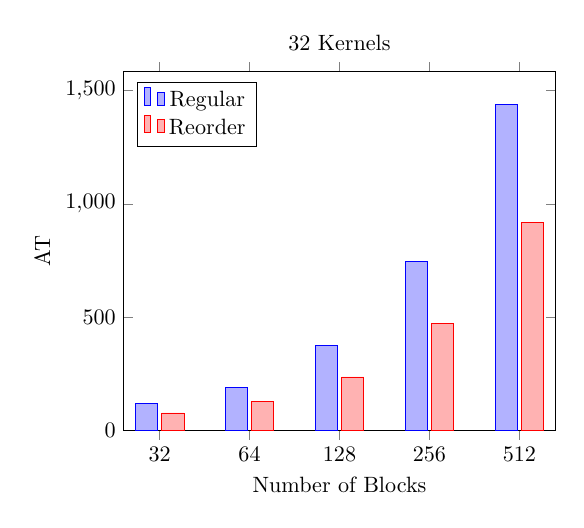
\begin{tikzpicture}[scale=0.80]
 \begin{axis}[
    title={32 Kernels},
    ymin=0,
    xtick=data,
    symbolic x coords={32,64,128,256,512},
	ylabel=AT,
	xlabel=Number of Blocks,
	legend pos=north west,
	ybar,
 ]
  \addplot coordinates {
(32,   116 )
(64,   190 )
(128,  374 )
(256,  744 )
(512,  1440)
};
  \addplot coordinates {
(32,   76  )
(64,   126 )
(128,  235 )
(256,  473 )
(512,  917 )
};
  \legend{Regular, Reorder}
 \end{axis}
\end{tikzpicture}
\end{center}
\caption{AT results for $N=32$.}
\label{fig:32kernels}
\end{figure}

\begin{figure}[htb]
\begin{center}
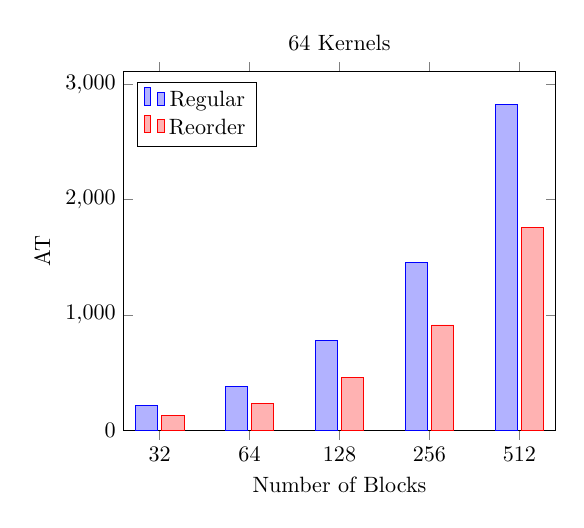
\begin{tikzpicture}[scale=0.80]
 \begin{axis}[
    title={64 Kernels},
    ymin=0,
    xtick=data,
    symbolic x coords={32,64,128,256,512},
	ylabel=AT,
	xlabel=Number of Blocks,
	legend pos=north west,
	ybar,
 ]
  \addplot coordinates {
(32,   211 )
(64,   383 )
(128,  777 )
(256,  1451)
(512,  2826)
};
  \addplot coordinates {
(32,   128 )
(64,   233 )
(128,  460 )
(256,  912 )
(512,  1758)
};
  \legend{Regular, Reorder}
 \end{axis}
\end{tikzpicture}
\end{center}
\caption{AT results for $N=64$.}
\label{fig:64kernels}
\end{figure}

\begin{figure}[htb]
\begin{center}
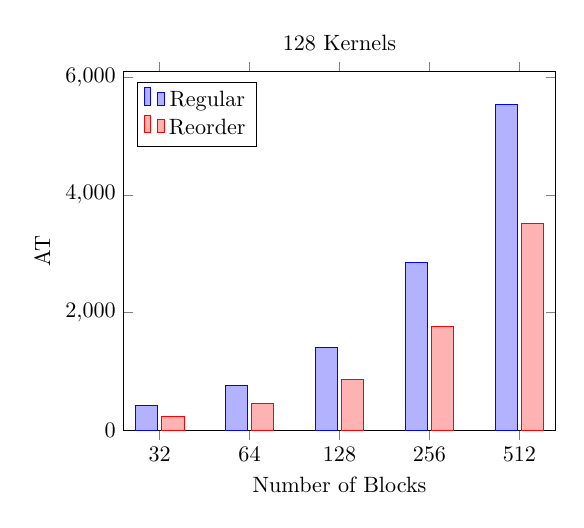
\begin{tikzpicture}[scale=0.80]
 \begin{axis}[
    title={128 Kernels},
    ymin=0,
    xtick=data,
    symbolic x coords={32,64,128,256,512},
	ylabel=AT,
	xlabel=Number of Blocks,
	legend pos=north west,
	ybar,
 ]
  \addplot coordinates {
(32,   416 )
(64,   762 )
(128,  1405)
(256,  2848)
(512,  5545)
};
  \addplot coordinates {
(32,   235 )
(64,   452 )
(128,  870 )
(256,  1763)
(512,  3512)
};
  \legend{Regular, Reorder}
 \end{axis}
\end{tikzpicture}
\end{center}
\caption{AT results for $N=128$.}
\label{fig:128kernels}
\end{figure}

\begin{figure}[htb]
\begin{center}
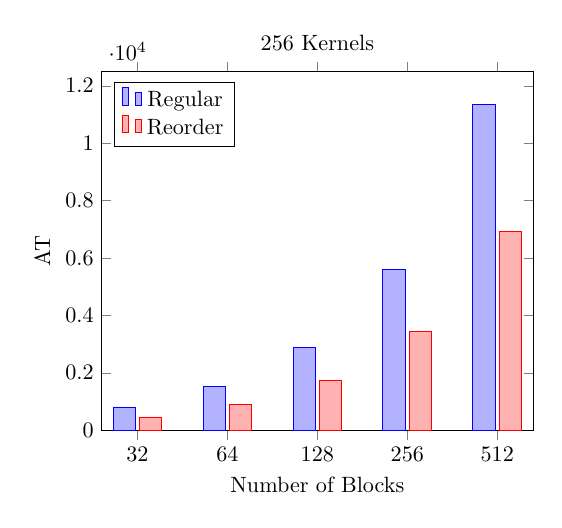
\begin{tikzpicture}[scale=0.80]
 \begin{axis}[
    title={256 Kernels},
    ymin=0,
    xtick=data,
    symbolic x coords={32,64,128,256,512},
	ylabel=AT,
	xlabel=Number of Blocks,
	legend pos=north west,
	ybar,
 ]
  \addplot coordinates {
(32,   810  )
(64,   1508 )
(128,  2876 )
(256,  5608 )
(512,  11363)
};
  \addplot coordinates {
(32,   461 )
(64,   888 )
(128,  1726)
(256,  3436)
(512,  6933)
};
  \legend{Regular, Reorder}
 \end{axis}
\end{tikzpicture}
\end{center}
\caption{AT results for $N=256$.}
\label{fig:256kernels}
\end{figure}

\subsection{Effects of the Kernel Value Computation}

In the knapsack problem, the values of the items to be put into the knapsack have a huge impact on the solution of the problem. One important contribution of this work is in the computation of $v_i$ (equation \eqref{eq:value}). In this computation, we consider the average percentage of resource requirements and the estimated time. We focus on increasing the value of kernels with greater resource requirements but shorter execution times. In scheduling, giving priority to jobs with shorter execution times reduces the average waiting time.

In order to evaluate the impact of the kernel value computation on the average waiting time, we implement two schemes for computing $v_i$: (i) as proposed in equation \eqref{eq:value}, called \textit{time}; and (ii) using only the average of the required resources, i.e., removing $t^{est}_i$ from equation \eqref{eq:value}, called  \textit{resources}.

% [bernardo]: Acho legal comentar que nem sempre é possivel ter o tempo estimado de um kernel. Nesse momento, é interessante desconsiderar o tempo e usar o grafico AWT sem tempo que gera um resultado interessante e depois dessa rodada, o valor do tempo pode ser considerado melhorando o resultado nas futuras execuções. Dessa forma, a cada vez que é executado o kernel, melhor irá ficar o tempo estimado em função do historico de execução e mais próximo irá ficar do a linha "time" no gráfico AWT.

Figure~\ref{fig:awt} shows the AWT for reordering submissions for $N \in \{32,64,128,256\}$ and $NB = 256$, considering the two different possibilities for computing $v_i$, \textit{time} and \textit{resources}. We can observe in this graph that the use of the estimated execution time in the computation of $v_i$ has a  positive impact on the AWT. The waiting time reduces from XXX to XXX compared to the \textit{resources} computation. Nevertheless, both computation modes of $v_i$ provide significant waiting time reductions when compared to Regular execution.  

\begin{figure}[htb]
\begin{center}
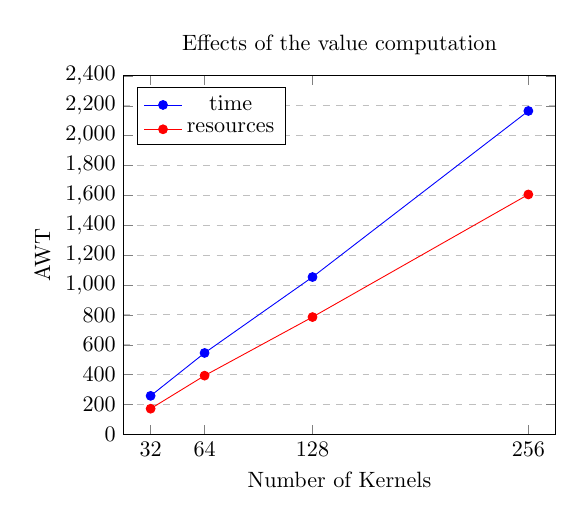
\begin{tikzpicture}[scale=0.80]
 \begin{axis}[
    title={Effects of the value computation},
    xlabel={Number of Kernels},
    ylabel={AWT},
    xmin=16, xmax=272,
    ymin=0, ymax=2400,
    xtick={32,64,128,256},
    ytick={0,200,400,600,800,1000,1200,1400,1600,1800,2000,2200,2400},
    legend pos=north west,
    ymajorgrids=true,
    grid style=dashed,
 ]
  \addplot[
    color=blue,
    mark=*,
    ] coordinates {
(32,258.459)
(64,545.556)
(128,1053.602)
(256,2165.010)
    };
  \addplot[
    color=red,
    mark=*,
    ] coordinates {
(32,172.477)
(64,393.831)
(128,785.808)
(256,1606.208)
    };
  \legend{time, resources}
 \end{axis}
\end{tikzpicture}
\end{center}
\caption{AWT results considering two forms to compute $v$, including the estimated time and using only the resource requirements.}
\label{fig:awt}
\end{figure}


\subsection{Overhead}

The kernel reordering is executed statically before the kernels are submitted to the GPU. Nevertheless, since the reordering computation involves solving a combinatorial optimization problem, we assess the overhead of the reordering algorithm.

Table~\ref{tab:overhead} shows the overhead of our reordering approach for $N \in \{32,64,128,256\}$ and $NB \in \{32,64,128,256,512\}$. The overhead is computed by comparing the execution time of the reordering algorithm with the absolute gain in the average execution time provided by reordering the kernels. If the reordering reduced the average execution time in 100 units of time and the reordering algorithm takes 10 units of time to execute, we consider the overhead of 10\%. This means that 10\% of our gains were spent on computing the solution.

% [bernardo]: O valor do overhead é inversamente proporcional ao tempo de duração dos kernels. Assim, kernels muito pequenos irao ter um overhead muito grande. Alem disso, dependendo da placa que ira ser executada, kernels grandes para uma K40 pode ser pequeno para um TitanX. Então, o valor do overhead está diretamente relacionada ao tempo da execução do kernel e o quanto rápido a placa que será executada é. Nos testes que realizamos, a média dos tempos dos kernels na TitanX é de 30 ms, mas já no K40 esse valor é bem maior. Isso justifica porque o overhead na k40 é muito pequeno e na TitanX é grande.

We can observe in Table~\ref{tab:overhead} that the overheads are low. We spent about XXX\% of our gains in the reordering scheme, which means that it is worth using a dynamic programming approach to reduce the average execution time. 

\begin{table}[htb]
    \centering
    \begin{tabular}{|c|c|c|c|c|c|} \hline
      & \multicolumn{5}{|c|}{NB}     \\ \cline{2-6}
 N    & 32  & 64  & 128  & 256 & 512 \\ \hline
 32   & 29  & 21  & 10   & 6.2 & 3.3 \\ \hline
 64   & 39  & 26  & 13   & 7.6 & 4.2 \\ \hline
 128  & 46  & 31  & 20   & 10  & 5.9 \\ \hline
 256  & 65  & 45  & 25   & 14  & 7.0 \\ \hline

    \end{tabular}
    \caption{Overhead of the reordering approach .}
    \label{tab:overhead}
\end{table}

\subsection{Portability}

Our reordering scheme is a software solution that can be applied to any NVIDIA GPU architecture that uses the Hyper-Q technology. The results reported so far clearly demonstrate the potential of the reordering scheme on the Maxwell architecture. We also evaluate our approach using a GPU based on the Kepler architecture. 

We report on Tables \ref{tab:32kernels-kepler} to \ref{tab:256kernels-kepler} the AT and STP results for the K40 GPU. As shown, our solution still achieves substantial reductions in AT and improvements in STP when compared to the Regular submissions. We obtain an average 34\% of reduction in AT and an average improvement in SP of XXx. Comparing with the TITAN-X results, we observe similar gains. This confirms that, although the two GPUs have different architecture features, our reordering scheme is performing well in taking advantage of the attainable resources provided.
 

\begin{table}[htb]
    \centering
    \begin{tabular}{|c|c|c|c|c|} \hline
      & \multicolumn{2}{|c|}{AT} & \multicolumn{2}{|c|}{STP} \\ \cline{2-5}
 NB   & Regular & Reorder & Regular & Reorder \\ \hline
 32   & 3084    & 2037           & 52      & 627            \\ \hline
 64   & 6782    & 3980           & 40      & 328            \\ \hline
 128  & 8997    & 6728           & 40      & 926            \\ \hline
 256  & 27812   & 15889          & 34      & 357            \\ \hline
 512  & 30432   & 15309          & 33      & 376            \\ \hline
    \end{tabular}
    \caption{Average Execution Time and STP results for the kernel set with 32 kernels.}
    \label{tab:32kernels-kepler}
\end{table}

\begin{table}[htb]
    \centering
    \begin{tabular}{|c|c|c|c|c|} \hline
      & \multicolumn{2}{|c|}{AT} & \multicolumn{2}{|c|}{STP} \\ \cline{2-5}
 NB   & Regular & Reorder & Regular & Reorder \\ \hline
 32   & 5709    & 3721           & 103     & 2361           \\ \hline
 64   & 8800    & 6262           & 90      & 880            \\ \hline
 128  & 20217   & 15066          & 78      & 902            \\ \hline
 256  & 33791   & 26004          & 69      & 691            \\ \hline
 512  & 117307  & 68703          & 65      & 1978           \\ \hline
    \end{tabular}
    \caption{Average Execution Time and STP results for the kernel set with 64 kernels.}
    \label{tab:64kernels-kepler}
\end{table}

\begin{table}[htb]
    \centering
    \begin{tabular}{|c|c|c|c|c|} \hline
      & \multicolumn{2}{|c|}{AT} & \multicolumn{2}{|c|}{STP} \\ \cline{2-5}
 NB   & Regular & Reorder & Regular & Reorder \\ \hline
 32   & 11753   & 6962           & 221     & 7856           \\ \hline
 64   & 22492   & 13354          & 171     & 7464           \\ \hline
 128  & 33472   & 25198          & 151     & 4245           \\ \hline
 256  & 78057   & 57377          & 140     & 6899           \\ \hline
 512  & 162713  & 111316         & 132     & 2782           \\ \hline
    \end{tabular}
    \caption{Average Execution Time and STP results for the kernel set with 128 kernels.}
    \label{tab:128kernels-kepler}
\end{table}

\begin{table}[htb]
    \centering
    \begin{tabular}{|c|c|c|c|c|} \hline
      & \multicolumn{2}{|c|}{AT} & \multicolumn{2}{|c|}{STP} \\ \cline{2-5}
 NB   & Regular & Reorder & Regular & Reorder \\ \hline
 32   & 26481   & 13214          & 407     & 25756          \\ \hline
 64   & 45018   & 30101          & 342     & 17852          \\ \hline
 128  & 96375   & 75247          & 297     & 13275          \\ \hline
 256  & 165133  & 109211         & 277     & 11418          \\ \hline
 512  & 311420  & 212702         & 297     & 9074           \\ \hline
    \end{tabular}
    \caption{Average Execution Time and STP results for the kernel set with 256 kernels.}
    \label{tab:256kernels-kepler}
\end{table}

\begin{table}[htb]
    \centering
    \begin{tabular}{|c|c|c|c|c|c|} \hline
      & \multicolumn{5}{|c|}{NB}     \\ \cline{2-6}
 N    & 32  & 64  & 128  & 256 & 512 \\ \hline
 32   & 0.984 & 0.287 & 0.133 & 0.025 & 0.025 \\ \hline
 64   & 1.212 & 0.278 & 0.195 & 0.077 & 0.014 \\ \hline
 128  & 0.482 & 0.230 & 0.266 & 0.111 & 0.045 \\ \hline
 256  & 0.536 & 0.638 & 0.431 & 0.141 & 0.078 \\ \hline

    \end{tabular}
    \caption{Overhead of the reordering approach .}
    \label{tab:overhead-kepler}
\end{table}

\section{Conclusions}
\label{sec:Conclusions}

As the GPU hardware continues to evolve, offering an increasingly amount of resources, it is very likely that in the future the GPU will move towards a multiprogrammed device. In this scenario, sharing the GPU resources is key to improve the overall computational throughput.


In this work, we propose a software  an optimization strategy that determines the order to submit the kernels for the GPU queues. The idea is to simulate the assignment of kernels to the hardware queues in order to maximize the resources utilization, improving the overall throughput. Our approach models the problem of selecting which kernels are better to submit to take the most advantage of the available resources as a series of knapsack problems. We model the set of the available resources as the knapsack capacity and the set of kernels as the items to be put into the knapsack. The kernels have weights and values 
according to the amount of resource usage -- shared memory, number of register and number of threads -- and the estimated execution time. The solution to the knapsack problem establishes the subset of kernels whose total weight is smaller than the available resources and the total value is as large as possible. We use a dynamic programming algorithm to solve the knapsack problem and the algorithm outputs a reordering of the kernel submissions that maximizes the resource utilization. Our reordering algorithm targets applications composed on many “heavy” kernels (i.e. kernels with large computational time) that have different resources requirements. For this reason, the combinatorial optimization problem we are facing has a limited number of items and executes in negligible time.  We present results XXX.

\section*{Acknowledgment}




\bibliographystyle{IEEEtran}
\nocite{*}
\bibliography{IEEEabrv,BiblioDB}

% that's all folks
\end{document}


%For comparison purpose, we also run the experiments with two different configurations, which we denominate as linear and greed. The linear represents the case were the kernels are executed in the same order they were submitted. The greed case corresponds to sort all the kernels according to the value $v_i$ achieved by equation \ref{Eq:value} in a decreased order. After sorted, the greed strategy calls the first kernel which fits in the device resource. This is made in a similar way than proposed by Li~\cite{li2015power}, although in this work the authors have different purposes and intends to schedule based on a complementary strategy on available device resources. 


%\subsection{Experimental Results}

% \begin{table}[htb]
%  \centering
%  \begin{tabular}{|c|c|c|c|c|} \hline
%      & \multicolumn{2}{|c|}{Average Waiting Time} 
%      & \multicolumn{2}{|c|}{Average Execution Time} \\ \cline{2-5}
%  NB  & Regular & Reorder & Regular & Reorder  \\ \hline
%  32  & 81.0    & 79.2    & 114.1   & 107.1    \\ \hline
%  64  & 180.1   & 135.4   & 219.9   & 167.9    \\ \hline
%  128 & 314.2   & 211.4   & 362.6   & 253.6    \\ \hline
%  256 & 666.9   & 415.8   & 737.1   & 480.6    \\ \hline
%  512 & 1337.7  & 819.3   & 1453.3  & 929.5    \\ \hline
%  \end{tabular}
%  \caption{TITAN-X results for the kernel set with 32 kernels in milisegs.}
%  \label{tab:AverageWaiting32Kernels}
% \end{table}

% \begin{table}[htb]
%  \centering
%  \begin{tabular}{|c|c|c|c|c|} \hline
%      & \multicolumn{2}{|c|}{Average Waiting Time} 
%      & \multicolumn{2}{|c|}{Average Execution Time} \\ \cline{2-5}
%  NB  & Regular & Reorder & Regular & Reorder  \\ \hline
%  32  & 187.7   & 169.1   & 222.2   & 198.2    \\ \hline
%  64  & 349.6   & 257.6   & 389.1   & 290.4    \\ \hline
%  128 & 703.6   & 470.8   & 754.1   & 515.4    \\ \hline
%  256 & 1388.5  & 876.1   & 1461.2  & 943.3    \\ \hline
%  512 & 2708.8  & 1644.3  & 2823.7  & 1753.5   \\ \hline
%  \end{tabular}
%  \caption{TITAN-X results for the kernel set with 64 kernels in milisegs.}
%  \label{tab:AverageWaiting64Kernels}
% \end{table}

% \begin{table}[htb]
%  \centering
%  \begin{tabular}{|c|c|c|c|c|} \hline
%      & \multicolumn{2}{|c|}{Average Waiting Time} 
%      & \multicolumn{2}{|c|}{Average Execution Time} \\ \cline{2-5}
%  NB  & Regular & Reorder & Regular & Reorder  \\ \hline
%  32  & 378.8   & 324.1   & 412.5   & 352.9    \\ \hline
%  64  & 722.4   & 516.9   & 761.6   & 550.2    \\ \hline
%  128 & 1493.1  & 963.8   & 1544.5  & 1009.5   \\ \hline
%  256 & 2847.8  & 1766.8  & 2920.9  & 1834.5   \\ \hline
%  512 & 5462.1  & 3358.5  & 5576.2  & 3467.3   \\ \hline
%  \end{tabular}
%  \caption{TITAN-X results for the kernel set with 128 kernels in milisegs.}
%  \label{tab:AverageWaiting128Kernels}
% \end{table}

% \begin{table}[htb]
%  \centering
%  \begin{tabular}{|c|c|c|c|c|} \hline
%      & \multicolumn{2}{|c|}{Average Waiting Time} 
%      & \multicolumn{2}{|c|}{Average Execution Time} \\ \cline{2-5}
%  NB  & Regular & Reorder & Regular & Reorder  \\ \hline
%  32  & 769.1   & 656.1   & 803.0   & 685.1    \\ \hline
%  64  & 1512.1  & 1076.7  & 1551.9  & 1110.8   \\ \hline
%  128 & 2860.4  & 1898.6  & 2910.7  & 1943.9   \\ \hline
%  256 & 5654.7  & 3618.9  & 5727.3  & 3686.7   \\ \hline
%  512 & 11045.3 & 6852.4  & 11160.1 & 6962.1   \\ \hline
%  \end{tabular}
%  \caption{TITAN-X results for the kernel set with 256 kernels in milisegs.}
%  \label{tab:AverageWaiting256Kernels}
% \end{table}


% \begin{itemize}
%     \item ``algoritmo (algoritmo de programacao dinamica, YYY), as variaveis, pesos''
%     \item ``tempo e a programacao dinamica.''
%     \item ``ajuste de pesos''
% \end{itemize}

%\begin{thebibliography}{1}
%\bibitem{IEEEhowto:kopka}
%H.~Kopka and P.~W. Daly, \emph{A Guide to \LaTeX}, 3rd~ed.\hskip 1em plus
%  0.5em minus 0.4em\relax Harlow, England: Addison-Wesley, 1999.
%\end{thebibliography}

% \begin{tikzpicture} 
%  \begin{axis}[
%   xlabel=n\textordmasculine Blocks,
%   ylabel=n\textordmasculine Kernels,
%   view/az=14
%  ] 
%   \addplot3[red,mark=*] coordinates {(32,32,829) (64,32,1503) (128,32,2833) (256,32,5608) (512,32,11143)}; 
%   \addplot3[red,mark=o] coordinates {(32,32,471) (64,32,961) (128,32,1828) (256,32,3562) (512,32,7226)}; 
%   \addplot3[green,mark=*] coordinates {(32,64,829) (64,64,1503) (128,64,2833) (256,64,5608) (512,64,11143)}; 
%   \addplot3[green,mark=o] coordinates {(32,64,471) (64,64,961) (128,64,1828) (256,64,3562) (512,64,7226)}; 
%   \addplot3[blue,mark=*] coordinates {(32,128,829) (64,128,1503) (128,128,2833) (256,128,5608) (512,128,11143)}; 
%   \addplot3[blue,mark=o] coordinates {(32,128,471) (64,128,961) (128,128,1828) (256,128,3562) (512,128,7226)}; 
%   \addplot3[yellow,mark=*] coordinates {(32,256,829) (64,256,1503) (128,256,2833) (256,256,5608) (512,256,11143)}; 
%   \addplot3[yellow,mark=o] coordinates {(32,256,471) (64,256,961) (128,256,1828) (256,256,3562) (512,256,7226)}; 
%  \end{axis} 
% \end{tikzpicture}

%Our performance analysis consisted on 4 groups of experiments, with a specified number of kernel launch in each of them. Table XXX shows the results, in milliseconds, of the total time consumed for their complete execution in each one of the cases: linear, greed and our dynamic approach. In each experiment we vary the maximum number of blocks created for each kernel. We remark that this total number does not correspond to the exact number but the upper limit allowed for each kernel launch. In this sense, we create random and real situations, where kernels can have very different number of blocks among them. We started with maximum of 8 blocks for kernel, since in real situation is not common to use less than this number.

%Since each experiment set generates random kernels, we executed 50 times all the experiments and uses the mean value of the final times, in order to minimize the random factor upcoming from the kernels.  

\begin{table}[htb]
    \centering
    \begin{tabular}{|c|c|c|c|c|} \hline
      & \multicolumn{2}{|c|}{Average Execution Time} & \multicolumn{2}{|c|}{STP} \\ \cline{2-5}
 NB   & Regular & Reorder & Regular & Reorder \\ \hline
 32   & 111     & 70             & 140     & 774            \\ \hline
 64   & 174     & 123            & 81      & 615            \\ \hline
 128  & 457     & 309            & 48      & 616            \\ \hline
 256  & 754     & 497            & 42      & 733            \\ \hline
 512  & 1421    & 931            & 36      & 661            \\ \hline
    \end{tabular}
    \caption{Average Execution Time and STP results for the kernel set with 32 kernels.}
    \label{tab:32kernels-titan}
\end{table}

\begin{table}[htb]
    \centering
    \begin{tabular}{|c|c|c|c|c|} \hline
      & \multicolumn{2}{|c|}{Average Execution Time} & \multicolumn{2}{|c|}{STP} \\ \cline{2-5}
 NB   & Regular & Reorder & Regular & Reorder \\ \hline
 32   & 220     & 129            & 250     & 2421           \\ \hline
 64   & 373     & 242            & 161     & 1785           \\ \hline
 128  & 799     & 569            & 106     & 2698           \\ \hline
 256  & 1385    & 904            & 85      & 1530           \\ \hline
 512  & 2477    & 1731           & 74      & 2152           \\ \hline
    \end{tabular}
    \caption{Average Execution Time and STP results for the kernel set with 64 kernels.}
    \label{tab:64kernels-titan}
\end{table}

\begin{table}[htb]
    \centering
    \begin{tabular}{|c|c|c|c|c|} \hline
      & \multicolumn{2}{|c|}{Average Execution Time} & \multicolumn{2}{|c|}{STP} \\ \cline{2-5}
 NB   & Regular & Reorder & Regular & Reorder \\ \hline
 32   & 413     & 235            & 612     & 10025          \\ \hline
 64   & 726     & 487            & 328     & 5366           \\ \hline
 128  & 1387    & 923            & 223     & 5117           \\ \hline
 256  & 2854    & 1862           & 170     & 4341           \\ \hline
 512  & 5585    & 3615           & 149     & 5145           \\ \hline
    \end{tabular}
    \caption{Average Execution Time and STP results for the kernel set with 128 kernels.}
    \label{tab:128kernels-titan}
\end{table}

\begin{table}[htb]
    \centering
    \begin{tabular}{|c|c|c|c|c|} \hline
      & \multicolumn{2}{|c|}{Average Execution Time} & \multicolumn{2}{|c|}{STP} \\ \cline{2-5}
 NB   & Regular & Reorder & Regular & Reorder \\ \hline
 32   & 829     & 471            & 1145    & 29565          \\ \hline
 64   & 1503    & 961            & 632     & 17910          \\ \hline
 128  & 2833    & 1828           & 438     & 13107          \\ \hline
 256  & 5608    & 3562           & 334     & 14743          \\ \hline
 512  & 11143   & 7226           & 291     & 15191          \\ \hline
    \end{tabular}
    \caption{Average Execution Time and STP results for the kernel set with 256 kernels.}
    \label{tab:256kernels-titan}
\end{table}

In order to produce the scheduling, SKonGP receives as input:  available GPU resources; and  required GPU  resources  and estimated execution time  per kernel.

The proposed scheduler associates a value, called $priority$,  per kernel, calculated as follows:

$priority = (GR / KR + GSM / KSM + GT / KT) / T$, where  $GR$, $GSM$ and $GT$ represent the number of registers, the  shared memory size in bytes and  the number of threads  available or supported by  a SM of a GPU  board, respectively; while  $KR$, $KSM$ and $KT$ represent the  corresponding required resources by the kernel. The estimated execution time of the kernel is given by $T$. Remark that, by using $priority$ to order the kernels,  our algorithm will favour the  execution of  kernels with the smallest requirements of resources and/or times.

SKonGP executes in  two steps. In the first one, called here InKerAssign, it creates  a group of kernels  that can be executed concurrently based on  $priority$.  Our   scheduler  produces this  initial group of kernels that will execute concurrently at each SM. In the second step, for each SM, the kernel with the smallest execution time is searched in the previous created group. The algorithm calculates the resources released by it, and try to schedule new kernels, by using the same algorithm of the previous step. The scheduler repeats this step until all kernel have  being scheduled.

The algorithm proposed for generating a initial assignment of kernels to a SM is inspired in the Knapsack Problem. The Knapsack Problem is a  well-known NP-hard  problem that has received a lot of attention from the researches. It  derives its name from the problem faced by someone who is constrained by a fixed-size knapsack and must fill it with the most valuable items,  respecting the  limited capacity of the knapsack \cite{Martello}.
 XXXXX colocar essas referencia no bibtex: S. Martello, P. Toth, Knapsack Problems: Algorithms and Computer Implementation, John Wiley and Sons, 1990. In our problem, we consider each SM  as a knapsack and the kernels as the itenms to be included  (assigned) in the knapsack (SM). However, here,  we consider the limit of  several types of  resources (registers, shared memory and threads)  and all threads have the same "value".



The Algorithm \ref{InKerAssign} receives, as input, the resources of the GPU board, called  GPUGlobal, and the list of  kernels to be scheduled, named ListKernel; and outputs a vector, named VecSM, where each position represents a SM and  contains a pointer to  a list of  kernels that will be assigned to it and the corresponding stream of each kernel. The loop in Algorithm \ref{alg1} is repeated N times, where N is the number of  SMs of the GPU board. XXX  explicar em linhas gerais o algoritmo e depois explicar o algoritmo linha a linha,  voce pode explicar  as variaveis  usadas por exemplo:  we consider that each kernel $K_i$ requires a number of registers $R_i$, a number of bytes in  shared memory $SM_i$ and  executes a number of threads $TH_i$. 

